\chapter{Technical and practical requirements}\label{chap:requirements}


\section{Input data}\label{sec:input_data}

	Information about potential unknown objects are passed to the program in the form of input files. There are two formats of files which contain relevant metadata, such as right ascension, declination, magnitude, and other, which are vital to the correct functioning of algorithms of tracklet building described in detail in chapter \ref{chap:proposed_solutions}. 
	
	The first is Flexible Image Transport System (FITS), a standardised and the most commonly used digital file format in astronomy. The second is an output from previous stage of the pipeline, a .cat file. 
	
	The formats are described in length in sections \ref{sec:fits_files} and \ref{sec:cat_files} respectively.
	
\subsection{Flexible Image Transport System files}\label{sec:fits_files}
	
	FITS is the standard archival data format for astronomical data sets. 
	
	It was originally designed in year 1981 for transporting image data on magnetic tapes between research institutions. In year 1982, FITS was officially endorsed by International Astronomical Union (IAU) as the format for the interchange of astronomical data.
	
	FITS files in this thesis are used as a source of data about objects and for image stacking \citep{FITSdefinition}.
	
\subsubsection{File structure}

	FITS files consist of three main FITS Structures (structures):
	
	\begin{itemize}
		\item primary header and data unit (HDU, mandatory)
		\item conforming extensions (optional)
		\item other special records (optional).
	\end{itemize}
	
	In our case, all FITS Files contain only the primary HDU which is sometimes referred to as Basic FITS File or a Single Image FITS File.
	
	If used, a structure contains a higher than zero number of FITS Blocks (blocks), each with size of 2880 bytes. Primary HDU always starts with the first block and each following structure begins with a block starting right after the end of the last block of previous structure. Furthermore, the primary HDU and each extension HDU must contain non-zero number of 2880-byte FITS Header (header) blocks, which are mandatory, and an optional array of associated 2880-byte data blocks\citep{FITSdefinition}.
	
\subsubsection{Data arrays} 
	
	If not empty, primary data array has a size of $1 x 999$ and is represented by continuous stream of bits. Each data value in the array consists of a fixed number of bits which are given in the keyword \emph{BITPIX}. If length of data is shorter than length of final block, the difference is filled by setting all the trailing bits to zero \citep{FITSdefinition}.
	
	An example of a partial FITS Data array is shown in Figure \ref{fig:fits_data_array} below.
	
	\begin{figure}[H]
	\centering
	  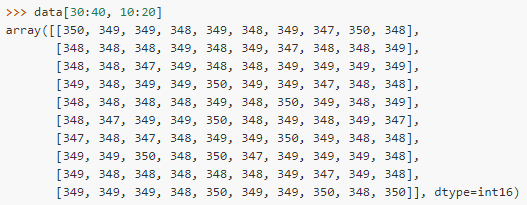
\includegraphics[width=10cm]{images/fits_data_array}
		  \caption{FITS data array represented as 2 byte integer in Python}
	  \label{fig:fits_data_array}
	\end{figure}
	
\subsubsection{Headers}

	Headers contain only limited set of text characters encoded in ASCII. Allowed characters are highlighted in Figure \ref{fig:allowed_ascii}.
	
	\begin{figure}[H]
	\centering
	  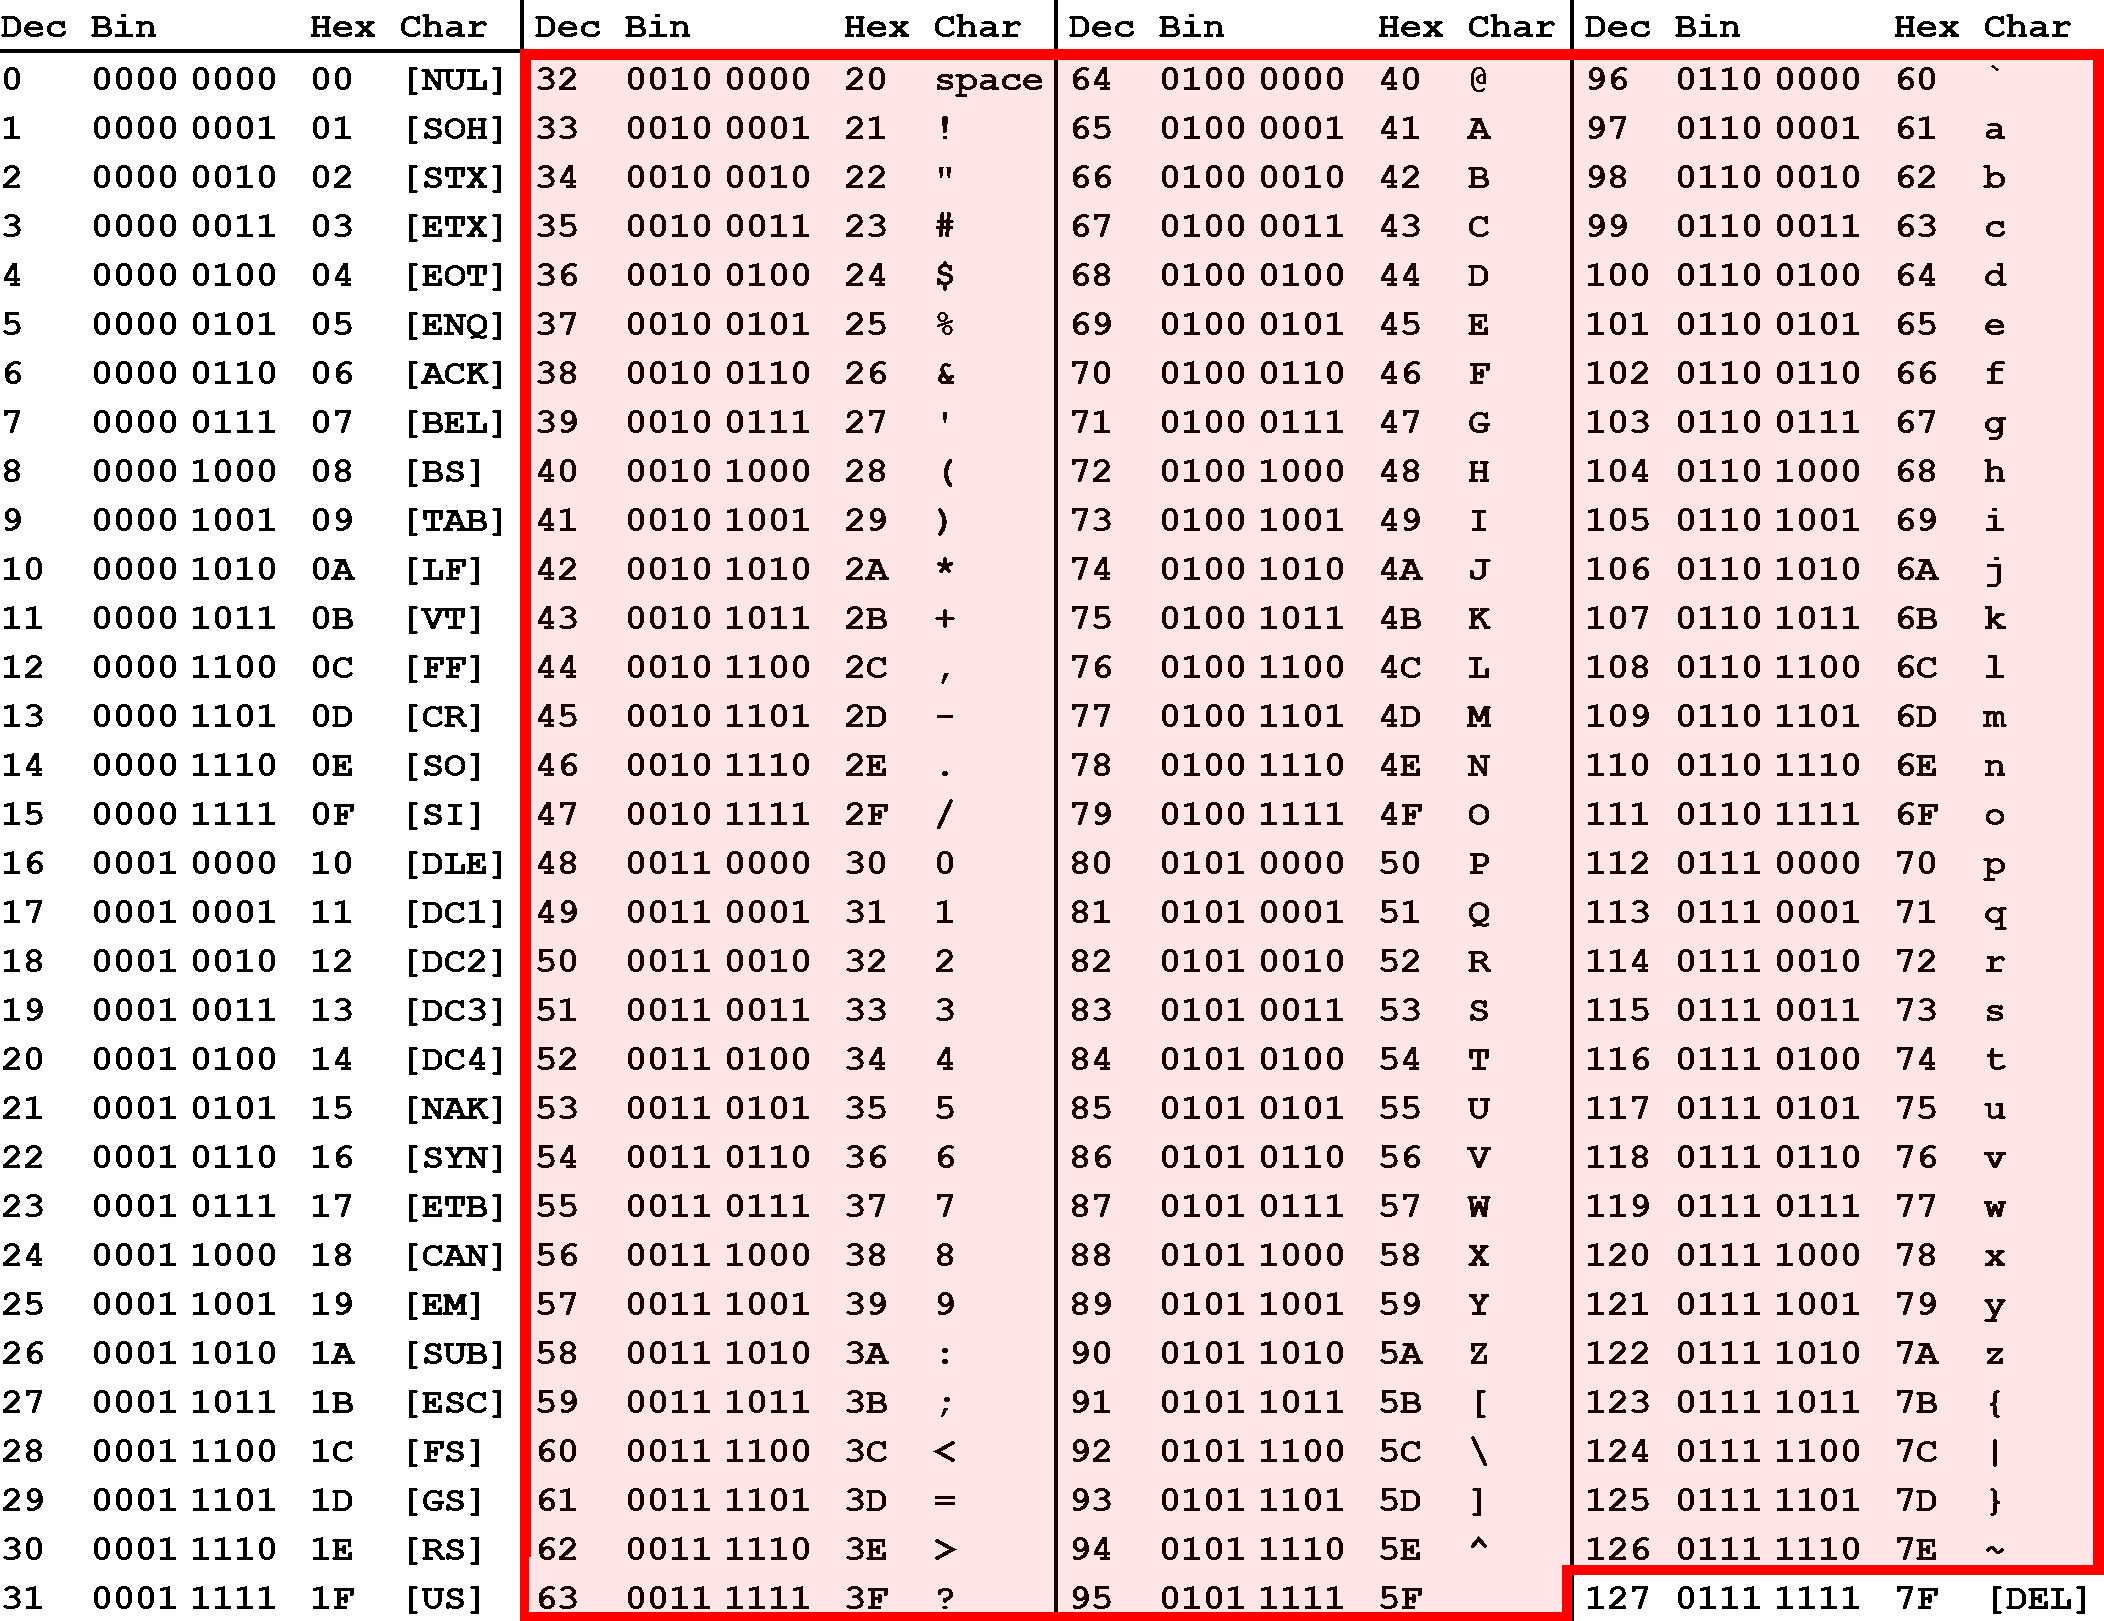
\includegraphics[width=10cm]{images/asciifull}
		  \caption{Allowed ASCII characters}
	  \label{fig:allowed_ascii}
	\end{figure}
	
	A header contains at least one header block, each consisting of maximum 80-character keyword sequence. In the 2880-byte block, this puts the maximum number of records at 36. The logical end of the block is marked by the END keyword and if there is space left, it is filled with ASCII character for space.
	
	Keywords are composed of key-value pairs and an optional comment. The presence of the value indicator (\emph{'= '}, ASCII character "equals" followed by ASCII character for space) determines that the key has a value associated with it. The values field can hold any of the following types:
	
	\begin{itemize}
		\item character string (eg. '27/10/82')
		\item logical value (represented as \emph{T} or \emph{F})
		\item integer number (eg. $12$)
		\item real floating-point number (eg. $-12.5$)
		\item complex integer number (eg. $2+4i$)
		\item complex floating-point number (eg. $7.8+1.7i$).
	\end{itemize}
	
	 Each FITS file (file) must contain several mandatory keywords (such as \emph{SIMPLE} - describes whether FITS file is a Basic Fits File or not; and other) which are reserved and have fixed types of their values. FITS format also contains reserved keywords that are not mandatory (such as \emph{DATE} - date on which the HDU was created, and other).
	 
	 In our case, the most relevant keywords are \emph{DATE-OBS} and \emph{EXPTIME}, or \emph{EXPOSURE} in files where the keyword \emph{EXPTIME} is missing \citep{FITSdefinition}.
	 
	 An example of FITS Header is shown in Figure \ref{fig:fits_header}.
	
	\begin{figure}[H]
	\centering
	  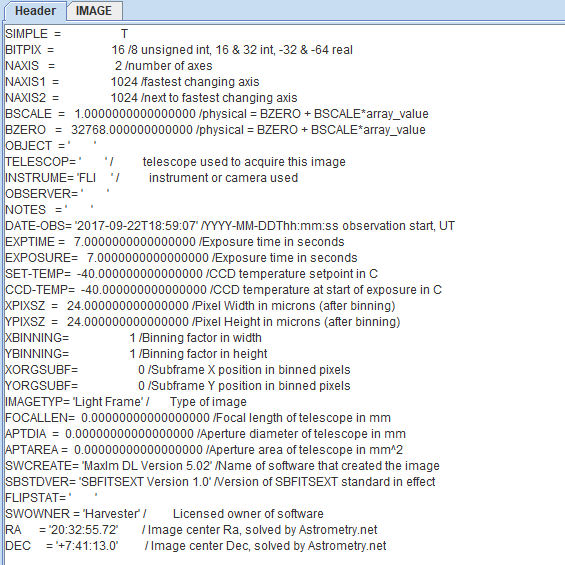
\includegraphics[width=10cm]{images/fits_header_example}
		  \caption{FITS Header example}
	  \label{fig:fits_header}
	\end{figure}

\subsection{.cat files}\label{sec:cat_files}
	
	.cat files are text files generated by the Astrometrica tool accepting FITS files (see \ref{sec:fits_files}) as input, providing interactive graphical user interface to manipulate each FITS file and performs image processing, segmentation, and astrometrical reduction resulting in an output file with the extension .cat.
	
	 Detailed description of the contents of a .cat file is in the following subsection.
	
\subsubsection{Contents of a .cat file}\label{subsubsec:content_cat}
	
	First four lines of a .cat file are a header - first line is empty, second is the name of the column, third contains units in which are values in specific column represented, and fourth is a separator, as shown in Figure \ref{fig:cat_header}.
	
	\begin{figure}[H]
	  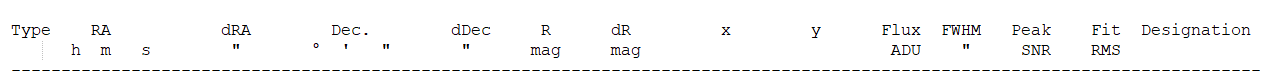
\includegraphics[width=\linewidth]{images/cat_columns}
		  \caption{.cat header columns}
	  \label{fig:cat_header}
	\end{figure}
	
	Meaning of each column is as follows:
	
	\begin{enumerate}
		\item Type - column outlining the type of a detected object; has four valid values:
		\begin{itemize}
			\item R - a star which has been matched with the star catalogue; if the value is in parentheses, the deviation between the two is too large
			\item H - a manually marked object
			\item S - a star which has not been matched with the star catalogue
			\item ? - an unknown object
		\end{itemize}
		\item RA - right ascension in hours/minutes/seconds (see Chapter \ref{chap:object_dynamics}, Section \ref{sec:ra_dec})
		\item dRA - deviation of values of RA between centroid created by Astrometrica and the star catalogue
		\item Dec. - declination in degrees/minutes/seconds (see Chapter \ref{chap:object_dynamics}, Section \ref{sec:ra_dec})
		\item dDec - deviation of values of DEC between centroid created by Astrometrica and the star catalogue
		\item R - brightness in magnitude
		\item dR - deviation of values of brightness between centroid created by Astrometrica and the star catalogue
		\item x - position of an object in FITS file on \emph{x} axis
		\item y - position of an object in FITS file on \emph{y} axis
		\item Flux - total intensity of all pixels in ADU (analog to digital unit)
		\item FWHM - "\emph{full width at half maximum}" describes a measurement of the width of a diffused object
		\item Peak - signal to noise ratio; describes the difference between the pixel with the maximal value and background
		\item Fit - the deviation of fitting of centroids in image to the star catalogue
		\item Designation - an user given input
	\end{enumerate}
	
\subsection{Processing server parameters}\label{sec:server_param}

	The server is a high CPU computer with Linux operating system capable of remote access for multiple users via console or x2goclient. The server is a Supermicro SuperServer 7048R-TR with an Intel\textsuperscript{\tiny\textregistered} Xeon\textsuperscript{\tiny\textregistered} E5-2640 v4 with Intel\textsuperscript{\tiny\textregistered} Turbo Boost Technology, hyper-threading and virtualization capabilities. It also contains 32GB of ECC DDR4 SDRAM 72-bit system memory, 400GB SSD system disk and 4TB SATA 3.0 HDD in RAID1 configuration for additional data storage. 920W power supply and free slots for an additional CPU, system memory sticks and GPUs provide for possible upgrade in the future.